
% \begin{frame}{Projective Metrics}{Motivation}
% 	\vspace{-1cm}
% 	\begin{itemize}
% 		\item Introduced by Gabidulin and Simonis (1997)\\~\\
% 		\item\uncover<2->{A \textbf{generalization} of many metrics in coding theory\\~\\}
% 		\item \uncover<3->{Related to (projective) \textbf{finite geometry}, \textbf{combinatorics}, \textbf{matroids}, \textbf{graph theory}, etc. \\~\\}
		
% 		\item \uncover<4->{\textbf{Sweet-spot} for research on metrics?\\~\\~\\}
% 	\end{itemize}

% \uncover<7->{

% \begin{center}
% \begin{tikzpicture}

% \uncover<5->{
% \draw (1,0.6) node[above] {Hamming};
% \draw (1,0)--(1,0.3) node[above] {metric};
% \draw (7.5,0.6) node[above] {Projective};
% \draw (7.5,0)--(7.5,0.3) node[above] {metrics};
% \draw (13,0.6) node[above] {Translation-invariant};
% \draw (13,0)--(13,0.3) node[above] {metrics};
% }
% \draw	
% (0,0)--(15,0);

% \draw (2.5,-0.1) node[below]  {$\leftarrow$	more specific/structured};
% \draw (15-1.5,-0.1) node[below]  { more general $\rightarrow$};
% \end{tikzpicture}
% \end{center}
% }

% \end{frame}
 %but first, let me tell you how i got interested in this topic

\begin{frame}{Projective Metrics}{Motivation}
	\vspace{-1cm}
	\begin{itemize}
		\item Introduced by Gabidulin and Simonis (1997)\\~\\ \
		\item \uncover<2->{A \textbf{generalization} of many metrics in coding theory\\~\\}
		
		
	\end{itemize}
\end{frame} 

 \begin{frame}{}{Projective metrics}
	
	Let $\cF = \{f_1,\ldots,f_N\} \subset V$ be a set of 
	such that $\langle f_1, f_2, \ldots, f_N \rangle = V$.\\~\\~\\

	\uncover<2->{
	The \textbf{projective weight function} $\wt_{\cF}(\cdot): V \to \mathbb{N}_{\geq 0}$ corresponding to  $\cF$ is 	
\[
\wt_{\cF}(x) := \min\{ t \in \mathbb{N}_{\geq 0} \,\,|\,\,  x \textnormal{ is in the linear span of } t \textnormal{ projective points } \langle f_i \rangle  \in \cF \}
\]
\text{}\\
}
\uncover<4->{
The \textbf{projective metric} $d_{\cF}(\cdot, \cdot): V \times V \to \mathbb{N}_{\geq 0}$ corresponding to $\cF$ is 	
\[
d_{\cF}(x,y) := \wt_{\cF}(y-x).
\]
}
\end{frame}


\begin{frame}{}{}
	\vspace{-1.5cm}
	Hamming metric
	\begin{equation*}
	\left(\begin{array}{c>{\columncolor{red!20}}ccc>{\columncolor{red!20}}cc>{\columncolor{red!20}}c}
	0  & 1  & 0 & 0 & 1 & 0 & 1\\
	\end{array}\right) \quad 	\uncover<2->{\to \; \cF = \cB \text{ the canonical basis.} }
	\end{equation*}
	
	\uncover<3->{
		Rank metric
		\begin{equation*}
		\left(\begin{array}{>{\columncolor{blue!20}}c>{\columncolor{blue!20}}c>{\columncolor{blue!20}}c}
		0  & 1  & 0 \\
		1  & 1  & 0 \\
		1  & 1  & 1 \\
		\end{array}\right)  \quad \uncover<4->{\to \; \cF = \{ \text{ rank 1 matrices} \}}
		\end{equation*}
	}
	
	
	\uncover<5->{
		Cover metric (rows and columns)
		\begin{equation*}
		\left(\begin{array}{c>{\columncolor{red!20}}cccc}
		0  & 1  & 0 & 0 & 0\\
		\rowcolor{red!20}
		0  & 1  & 0 & 1 & 1\\
		0  & 1  & 0 & 0 & 0\\
		\rowcolor{red!20}
		1  & 0  & 0 & 1  & 0\\
		\end{array}\right)  \quad \uncover<6->{\to \; \cF = \left\{ \text{matrices with 1  non-zero row or 1 non-zero column} \right\}}
		\end{equation*}
	}
	
	\uncover<7->{
		Phase-rotation metric
			\begin{equation*}
			\left(\begin{array}{cccc}
			1  & 1  & 0 & 1\\
			\end{array}\right) = \left(\begin{array}{cccc}
			\rowcolor{red!20}
			1  & 1  & 1 & 1\\
			\end{array}\right) + \left(\begin{array}{cc>{\columncolor{red!20}}cc}
			0  & 0 & 1 &  0\\
			\end{array}\right)  \quad  \uncover<8->{\to \; \cF = \left\{ \text{standard basis vectors or all-1} \right\}}
			\end{equation*}
	
	}

	\text{}\\~\\\text{}
\end{frame}


\contourlength{1.0pt}

\begin{frame}{}{}
\vspace{-5cm}
%\only<1-2>{\uncover<2-2>{Strongly regular Clebsch graph / Greenwood–Gleason graph}}
\only<1-1>{Vertices: vectors of $\F_2^4$}
\only<2-3>{Distance from $0000$ to $1101$: \uncover<3->{\textcolor{red}{red:} 3,} \uncover<4->{\textcolor{blue}{blue:} 2}}
%\only<7->{\textbf{Phase-rotation metric:} an edge is a Hamming error or the \alert{all-bits-flip error}}
\begin{center}
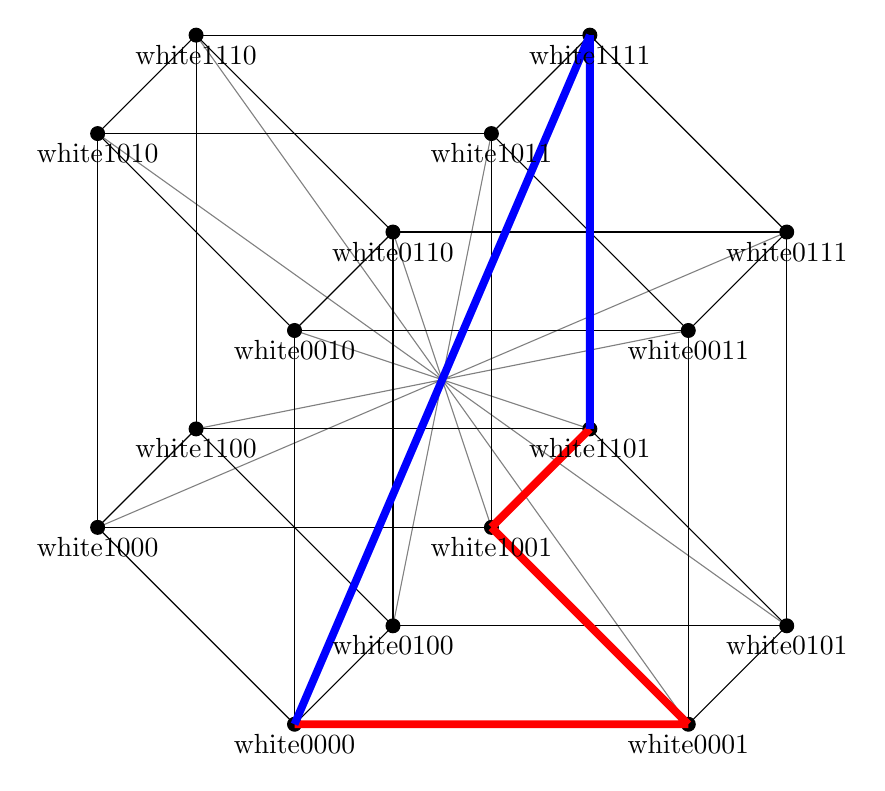
\begin{tikzpicture}[yscale=2.5, xscale=2.5, rotate=0]

\coordinate (0000) at (1,1);
\coordinate (0001) at (3,1);
\coordinate (0010) at (1,3);
\coordinate (0011) at (3,3);
\coordinate (0100) at (1.5,1.5);
\coordinate (0101) at (3.5,1.5);
\coordinate (0110) at (1.5,3.5);
\coordinate (0111) at (3.5,3.5);

\coordinate (1000) at (0,2);
\coordinate (1001) at (2,2);
\coordinate (1010) at (0,4);
\coordinate (1011) at (2,4);
\coordinate (1100) at (0.5,2.5);
\coordinate (1101) at (2.5,2.5);
\coordinate (1110) at (0.5,4.5);
\coordinate (1111) at (2.5,4.5);

\uncover<2->{
\draw[gray]
(0000) -- (1111)
(0010) -- (1101)
(0100) -- (1011)
(0110) -- (1001)
(1000) -- (0111)
(1010) -- (0101)
(1100) -- (0011)
(1110) -- (0001)
;
}

\draw
(0000) -- (0001)
(0010) -- (0011)
(0100) -- (0101)
(0110) -- (0111)
(1000) -- (1001)
(1010) -- (1011)
(1100) -- (1101)
(1110) -- (1111)
;


\draw
(0000) -- (0010)
(0001) -- (0011)
(0100) -- (0110)
(0101) -- (0111)
(1000) -- (1010)
(1001) -- (1011)
(1100) -- (1110)
(1101) -- (1111)
;

\draw
(0000) -- (0100)
(0001) -- (0101)
(0010) -- (0110)
(0011) -- (0111)
(1000) -- (1100)
(1001) -- (1101)
(1010) -- (1110)
(1011) -- (1111)
;

\draw
(0000) -- (1000)
(0001) -- (1001)
(0010) -- (1010)
(0011) -- (1011)
(0100) -- (1100)
(0101) -- (1101)
(0110) -- (1110)
(0111) -- (1111)
;




\filldraw[black] (0000)  circle (1pt);
\filldraw[black] (0001)  circle (1pt);
\filldraw[black] (0010)  circle (1pt);
\filldraw[black] (0011)  circle (1pt);
\filldraw[black] (0100)  circle (1pt);
\filldraw[black] (0101)  circle (1pt);
\filldraw[black] (0110)  circle (1pt);
\filldraw[black] (0111)  circle (1pt);

\filldraw[black] (1000)  circle (1pt);
\filldraw[black] (1001)  circle (1pt);
\filldraw[black] (1010)  circle (1pt);
\filldraw[black] (1011)  circle (1pt);
\filldraw[black] (1100)  circle (1pt);
\filldraw[black] (1101)  circle (1pt);
\filldraw[black] (1110)  circle (1pt);
\filldraw[black] (1111)  circle (1pt);


\uncover<3->{
	\draw[line width=1.0mm, red]
	(0000) -- (0001)
	(0001) -- (1001)
	(1001) -- (1101)
	;}

\uncover<4->{
	\draw[line width=1.0mm, blue]
	(0000) -- (1111)
	(1111) -- (1101)
	;}


\uncover<1->{

\draw (0000) node[below] {\contour{white}{0000}};
\draw (0001) node[below] {\contour{white}{0001}};
\draw (0010) node[below] {\contour{white}{0010}};
\draw (0011) node[below] {\contour{white}{0011}};
\draw (0100) node[below] {\contour{white}{0100}};
\draw (0101) node[below] {\contour{white}{0101}};
\draw (0110) node[below] {\contour{white}{0110}};
\draw (0111) node[below] {\contour{white}{0111}};

\draw (1000) node[below] {\contour{white}{1000}};
\draw (1001) node[below] {\contour{white}{1001}};
\draw (1010) node[below] {\contour{white}{1010}};
\draw (1011) node[below] {\contour{white}{1011}};
\draw (1100) node[below] {\contour{white}{1100}};
\draw (1101) node[below] {\contour{white}{1101}};
\draw (1110) node[below] {\contour{white}{1110}};
\draw (1111) node[below] {\contour{white}{1111}};
}




\end{tikzpicture}
\end{center}

\vspace{-5cm}
%\vspace{-10cm}
%\uncover<1-2>{\text{}\hspace{13cm}\includegraphics[scale=0.2]{clebsch3.png}}



\end{frame}






% \begin{frame}{Equivalent notions - 2 }{Subspace Arrangments}
%      For a set \(I \subset \cF\) let \(F_I \coloneqq \langle f \mid f \in I\rangle \). 
%     For \(t \in \bN\) consider the subspace arrangement \( \mathcal{A} \coloneqq \{F_I \mid dim(F_I) = t\}\). Then we have \(B_t(0) = \cup_{F_I \in \cA}F_I\). By exclusion/inclusion we have 
%     \begin{equation}
%         |B_t(0)| = \sum_{J \subset \cA} (-1)^{|J|+1}|\cap_{F \in J}F|
%     \end{equation}
%     An other version is obtained by considering the lattice: \(\cL_{\cA} \{\cap_{F \in J}F | J \subset \cA\}\) ordered by reverse inclusion.
%     \begin{equation}
%         |\bF^n_q \setminus B_t(0)|= \sum_{x \in \cL_{\cA}}\mu(\bF_q^n,x) card(x)
%     \end{equation}
%     Where \( \mu\) is the Möbius function of \(\cL_{\cA}\).

% \end{frame}

% \begin{frame}{Equivalent notions - 2 }{Subspace Arrangments}
% \begin{itemize}
% 	\item For some subspace arrangements the  Möbius function of some subspace arrangements is known.
% 	\item It may be useful to try to understand whether any of these can be induced by a projective metric. 
% 	\item This also points in the direction of trying to study the homology group of the lattice associated to a sphere of a projective metric.
% 	\item Ideas on how this might work are very welcome! :)
% \end{itemize}
% \end{frame}

% \begin{frame}{Equivalent notions - 3}{Known Hamming codes}
% 	A very important connection to Classical Coding theory is given by the following.
% 	\begin{definition}(Parent functions and Parent codes of $\cF$)
% 		The \myfont{parent functions} of $\cF$ are $\Ff_q$-linear functions $\varphi: \Ff_q^{\N} \to V$ such that $\langle \varphi( e_i ) \rangle = F_{\sigma(i)} \in \cF$ for some $\sigma(i) \in S_{\N}$.
% 		The \myfont{parent codes} of $\cF\subset \Gr_1(V)$ are the elements in the class $\bar \C := [\ker (\varphi)]$ where \([\ker (\varphi)]\) is the equivalence class of $\ker(\varphi)$ and \(\varphi\) is a parent function of $\cF$.
% 	\end{definition}

% Given \(v \in \cV\) the parent code \(\cC\) describes all the possible linear combinations of \(\cF\) that equal to \(v\).
% That is we have: \(v = \sum_{f \in \cF} a_ff = \sum_{f \in \cF} b_ff \) that is \(v = \varphi(a) = \varphi(b)\) if and only if \( a-b \in \cC\). 
% A series of important proprieties depends on this code, for example we have that:
% % \begin{observation}
% % \end{observation}
% If \(x \in \mathbb{F}_q^\mathbb{N}\) satisfies \(\wt_H(x) \leq \frac{d_H(\mathcal{C})}{2}\), then \(\wt_H(x) = \wt_\mathcal{F}(\varphi(x))\).


% \end{frame}








\begin{frame}{}{What can we do?}
\vspace{-1.5cm}
\uncover<2->{Singleton-type bound!\\~\\}

\uncover<4->{
\begin{definition*}
	\textnormal{
	Let $t \in \{0,1,2,\ldots,N\}$. We define $\mu_{\cF}(t)$ as the maximum cardinality of a subset $\cG \subseteq \cF$ satisfying
	\begin{enumerate}
		\item \uncover<5->{All $f_i \in \cG$ are linear independent from each other;}
		\item \uncover<6->{All $v \in \langle \cG \rangle$ have $\wt_{\cF}(v) \leq t$.}
	\end{enumerate}
}
\end{definition*}
}

\uncover<7->{
\begin{theorem}[\textbf{General Singleton-type bound}] 

 \scalebox{1.1}{Let $\C \subseteq V$ be a subset and let $d = \min\{d_{\cF}(x,y) \,|\, x \neq y \in \C)\}$. Then}
	\[
	\scalebox{1.2}{$|\C| \leq q^{N - \mu_{\cF}(d-1)} \leq q^{N-d+1}$
}
	\]
\end{theorem}
}

\uncover<8->{
	\textbf{Coincides} with Singleton bounds for specific projective metrics!
}
\end{frame}

\begin{frame}{Sketch of Proof}
    Write $\mu := \mu_{\mathcal{F}}(d-1)$ and let $\mathcal{G} = \{g_1, \ldots, g_\mu\} \subseteq \mathcal{F}$ be the linearly independent subset of size $\mu$ from the definition of \(\mu_{\mathcal{F}}(t)\). \pause (thus \(\mathrm{wt}_{\mathcal{F}}(\mathcal{\langle G \rangle}) \leq d-1\)).
    \pause % Adds a pause here
    We can extend $\mathcal{G}$ to a basis $\mathcal{B}$ for $V$:
    \[
    \mathcal{B} = \{g_1, \ldots, g_\mu, g_{\mu+1}, \ldots, g_{N}\}
    \]
    
    \pause % Adds a pause here
    Consider the projection:
    \begin{align*}
        \operatorname{Proj}: \mathcal{C} & \to \mathbb{F}_q^{N - \mu} \\
        \sum_{i=1}^{N} c_i g_i & \mapsto (c_{\mu+1}, \ldots, c_{N})
    \end{align*}
   \pause
   If \( \operatorname{Proj}\) is injective, then \(|\cC| \leq q^{N-\mu(d-1)}\) which is the Singleton Bound. \\ \pause 
    Let $a, b \in \mathcal{C}$ and suppose $\operatorname{Proj}(a) = \operatorname{Proj}(b)$. \pause Then $\operatorname{Proj}(a-b) = 0$, so $a - b \in \langle \mathcal{G} \rangle$. \pause But this means that
    \[
    d_{\mathcal{F}}(a,b) = \mathrm{wt}_{\mathcal{F}}(a - b) \leq d - 1 < d,
    \]
    so $a = b$.
\end{frame}


\begin{frame}{A deep connection to Classical Coding }{What can we do?}

Let \(\cF = \{ f_1,\ldots, f_{\N} \}\), consider: \pause
\begin{align}
	\varphi:\bF_q^{\N}&\to  V \\
	 e_i &\mapsto  f_i  
\end{align}
\pause % Optional pause before starting the content
$\varphi$ is called a \textbf{parent function} of $\wt_{\mathcal{F}}$ and 
\pause % Pause before revealing the next part
$\mathcal{P} := \ker(\varphi)$ is a \textbf{parent code} of $\wt_{\mathcal{F}}$.
\pause
\begin{theorem}
    \begin{align*}
    \Psi: \bar Pr_{\N}(V) &\to \bar Gr_{\N-N}(\Ff_q^{\N}) \\
    \bar w_{\cF} &\mapsto \bar \cP_{\cF}
	\end{align*}
    Where $ \bar Pr_{\N}(V)$ is the set containing the equivalence classes of projective metrics on $V$ of size $\N$ and $\bar Gr_{\N-N}(\Ff_q^{\N})$ be the set containing the equivalence classes of subspaces of $\Ff^{\N}_q$ of dimension $\N - N$.
\end{theorem}


\end{frame}

% \begin{frame}{Constructions}{What can we do?}
% \vspace{-1cm}
% \uncover<2->

% \uncover<3->{
% We can define
% \[
% \wt_{\cF} \cup \wt_{\cG} := \wt_{\cF \cup \cG}
% \]
%  and
% \[
% \wt_{\cF} \otimes \wt_{\cG} := \wt_{\cF \otimes \cG}
% \]
% where $\cF \otimes \cG := \{\langle f_i \rangle \otimes \langle g_i \rangle \,\,|\,\, \langle f_i \rangle \in \cF, \,\langle g_i \rangle \in \cG \}$\\~\\
% }

% \uncover<4->{
% \textbf{Example}\\

% Let $\cF = \{\text{all 1-dim subspaces of } V\}$. Then $\wt_{\cF}(x) = 1$ for all $x\neq 0$. This is the \textbf{discrete weight} $\wt_{\operatorname{Dis}}$.\\~\\
% }

% \uncover<5->{

% \textbf{Examples}\\
% \begin{itemize}
% 	\item \uncover<6->{
% 		\scalebox{1.2}{$\wt_{\operatorname{Dis}} \otimes \wt_{\operatorname{Dis}} = \wt_{\operatorname{Rank}}$} \\}%\,\,\,\, (on $V_1 \otimes V_2$)
% 	\item \uncover<7->{\scalebox{1.2}{$\wt_{\operatorname{H}} \otimes \wt_{\operatorname{Rank}} = \wt_{\operatorname{Sum-rank}}$}\\}
% 	\item\uncover<8->{ \scalebox{1.2}{$\wt_{\operatorname{Dis}} \otimes \wt_{\operatorname{H}} = \wt_{\operatorname{Row}}$}\\}
% 	\item \uncover<9->{\scalebox{1.2}{$\wt_{\operatorname{H}} \otimes \wt_{\operatorname{Dis}} = \wt_{\operatorname{Column}}$}\\}
% 	\item \uncover<10->{\scalebox{1.2}{$\wt_{\operatorname{Row}} \cup \wt_{\operatorname{Column}} = \wt_{\operatorname{Cover}}$}}
% \end{itemize}

% }
% \end{frame}

\begin{frame}{A connection to Classical Coding Theory}

\begin{definition}[Perfect codes]
    Given a distance function \(d\) on \(V\) and a code \(\cC \subseteq V\), we say that \(\cC\) is \textbf{perfect} with respect to \(d\) if there exists a \(t \in \bN\) such that:

    \begin{equation}
        \bigsqcup_{c \in \cC}B_t(c) = V
    \end{equation}
    where \(B_t(c) := \{x \in V : d(x,c) \leq t\}\) are disjoint balls of radius \(t\) centered around codewords.
  %  That is the balls of radious \(t\) centered on the codeword of \(\cC\) are disjoint and fill out the space.
\end{definition}
\pause
	\begin{proposition}
		A linear code \(\cC < V\) is \(\cF\)-perfect if and only if \(\varphi^{-1}(\cC)\) is Hamming perfect.
	 \end{proposition}
	 \pause
\textbf{Remark 1:} There is a complete characterization for Hamming perfect codes which could be leveraged for projective metrics. \\ 
\pause \textcolor{gray}{Which is kind of fun, because you are using one specific metric to get results on a class of metrics, containing the metric itself.}
\end{frame}

\begin{frame}{Characterization of projective isometries}{What can we do?}
    
\begin{definition}
	An \(\mathcal{F}\)-isometry is a linear isomorphism \(L:V \to V\) such that \(d_{\mathcal{F}}(Lx,Ly) = d_{\mathcal{F}}(x,y)\) for all \(x,y \in V\). \pause The set of \(\mathcal{F}\)-isometries, with the operation of composition, forms a group denoted as \(\mathrm{Isom}_{\mathcal{F}}(V)\).
\end{definition}

\pause 
\begin{theorem}
Let \(stab_H(\cP)\) be the stabilizer of the parent code \(\cP\) respect to the Hamming isometries, then \(isom_{\cF}(V) \cong stab_H(\cP)\)
\end{theorem}

% \begin{theorem}
%     \(isom_{\cF}(V) \cong stab_H(\C)\). The group isomorphism is given by \(\Psi: stab_H(\C) \to isom_{\cF}(V)\) where \(\Psi(F) = \hat F\), the unique \(\cF\)-isometry such that the following diagram commutes:
%     \[\begin{tikzcd}[ampersand replacement=\&]
%         V \arrow[r,"F"] \& V \\
%         \Ff_q^{\N} \arrow[u,"\varphi"] \arrow[r,"\hat F"'] \& \Ff_q^{\N} \arrow[u,"\varphi"']
%     \end{tikzcd}\]
% \end{theorem}
\end{frame}


\begin{frame}{}{Current research}
\vspace{-0.5cm}
\begin{itemize}
\item Algorithms for calculating  $\wt_{\cF}(v)$ for $v \in V$ 
\item \pause Are there general methods for obtaining sphere sizes $|\{v \in V \,|\, \wt_{\cF}(v)=t\}|$ for $t \in \mathbb{N}$?
\item \pause Is there a natural way do generalize other concepts of coding theory? Dual Codes? MDS Codes? ...
\item \pause New metrics from old?: using poset lattice of projective metrics, where $\wt_{\cF} \preccurlyeq \wt_{\cG} $ iff $\cF \subseteq \cG $
\end{itemize}

\pause
\begin{center}
	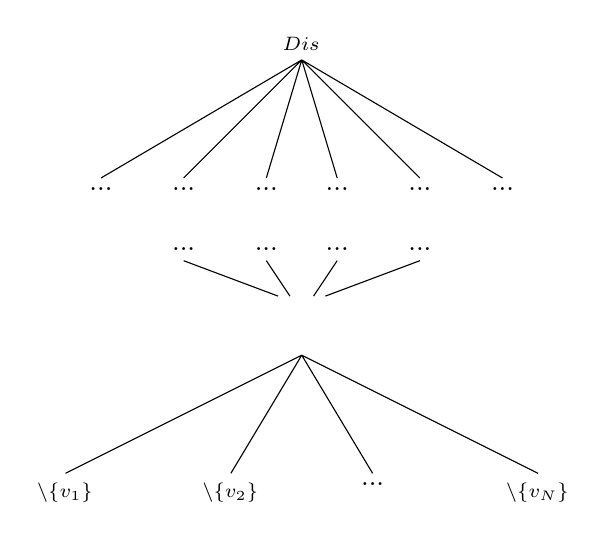
\begin{tikzpicture}[yscale=1.5, xscale=1.5, rotate=0]
	
	\draw (0,0) node[above] {$\wt_{\operatorname{Dis}}$}--(-1, -1) node[below] {...}
	(0,0) --(-0.3, -1) node[below] {...}
	(0,0) --(0.3, -1) node[below] {...}
	(0,0) --(1, -1) node[below] {...}
	(0,0) --(1.7, -1) node[below] {...}
	(0,0) --(-1.7, -1) node[below] {...}
	;
	
	
	\draw (0,-2.5) node[above] {$\wt_{\cF}$}--(-2, -3.5) node[below] {$\wt_{\cF \setminus \{v_1\}}$}
	(0,-2.5) --(-0.6, -3.5) node[below] {$\wt_{\cF \setminus \{v_2\}}$}
	(0,-2.5) --(0.6, -3.5) node[below] {...}
	(0,-2.5) --(2, -3.5) node[below] {$\wt_{\cF \setminus \{v_N\}}$}
	;
	
	\draw (-0.2,-2) -- (-1, -1.7) node[above] {...}
	(-0.1,-2) -- (-0.3, -1.7)  node[above] {...}
	(0.1,-2) -- (0.3, -1.7)  node[above] {...}
	(0.2,-2) -- (1, -1.7)  node[above] {...}
	;
	
\end{tikzpicture}
\end{center}



\end{frame}


\begin{frame}{Connections to Other Fields}
	{\pause (Of mathematics, not algebraic fields.)}

	\begin{itemize}
		\item \pause \textbf{Graph Theory:}\\
			The Cayley graph of \(\mathbb{F}_q^N\) with generating set \(\mathcal{F}\); \pause $\wt_{\mathcal{F}}(v)$ is the graph distance between \(v\) and \(0\).
		
		\item \pause \textbf{Classical Coding Theory:}\\
			The parent code \(\mathcal{P}\) of \(\wt_{\mathcal{F}}\).
		
		\item \pause \textbf{Projective Geometry:}\\
			The projective weights are constant on the projective classes of \(\mathbf{P}(V)\). \\ pause
			\pause And \(\wt_{\mathcal{F}}\)-isometries are simply homographies fixing \(\mathcal{F}\).
			
		\item \pause \textbf{Subspace Arrangements:} \\
			A ball of size \(t\) in projective metric corresponds to the size of the \textbf{subspace arrangement} generated by subsets of \(\mathcal{F}\) of size less than \(t\).     
			
		\item \pause \textbf{Matroid Theory:}\\
			We can observe the matroid associated with the family \(\mathcal{F}\). \pause This seems to describe well the first two layers of the intersection lattice.
			
	\end{itemize}
\end{frame}
	
\begin{frame}
	Thank you for your attention.	
\end{frame}